% Options for packages loaded elsewhere
\PassOptionsToPackage{unicode}{hyperref}
\PassOptionsToPackage{hyphens}{url}
%
\documentclass[
]{article}
\usepackage{lmodern}
\usepackage{amssymb,amsmath}
\usepackage{ifxetex,ifluatex}
\ifnum 0\ifxetex 1\fi\ifluatex 1\fi=0 % if pdftex
  \usepackage[T1]{fontenc}
  \usepackage[utf8]{inputenc}
  \usepackage{textcomp} % provide euro and other symbols
\else % if luatex or xetex
  \usepackage{unicode-math}
  \defaultfontfeatures{Scale=MatchLowercase}
  \defaultfontfeatures[\rmfamily]{Ligatures=TeX,Scale=1}
\fi
% Use upquote if available, for straight quotes in verbatim environments
\IfFileExists{upquote.sty}{\usepackage{upquote}}{}
\IfFileExists{microtype.sty}{% use microtype if available
  \usepackage[]{microtype}
  \UseMicrotypeSet[protrusion]{basicmath} % disable protrusion for tt fonts
}{}
\makeatletter
\@ifundefined{KOMAClassName}{% if non-KOMA class
  \IfFileExists{parskip.sty}{%
    \usepackage{parskip}
  }{% else
    \setlength{\parindent}{0pt}
    \setlength{\parskip}{6pt plus 2pt minus 1pt}}
}{% if KOMA class
  \KOMAoptions{parskip=half}}
\makeatother
\usepackage{xcolor}
\IfFileExists{xurl.sty}{\usepackage{xurl}}{} % add URL line breaks if available
\IfFileExists{bookmark.sty}{\usepackage{bookmark}}{\usepackage{hyperref}}
\hypersetup{
  pdftitle={Covid19 Response Ratio Comparison between Canada and USA},
  pdfauthor={Fatime Selimi, Neel Phaterpekar, Nicholas Wu, Tanmay Sharma},
  hidelinks,
  pdfcreator={LaTeX via pandoc}}
\urlstyle{same} % disable monospaced font for URLs
\usepackage[margin=1in]{geometry}
\usepackage{graphicx}
\makeatletter
\def\maxwidth{\ifdim\Gin@nat@width>\linewidth\linewidth\else\Gin@nat@width\fi}
\def\maxheight{\ifdim\Gin@nat@height>\textheight\textheight\else\Gin@nat@height\fi}
\makeatother
% Scale images if necessary, so that they will not overflow the page
% margins by default, and it is still possible to overwrite the defaults
% using explicit options in \includegraphics[width, height, ...]{}
\setkeys{Gin}{width=\maxwidth,height=\maxheight,keepaspectratio}
% Set default figure placement to htbp
\makeatletter
\def\fps@figure{htbp}
\makeatother
\setlength{\emergencystretch}{3em} % prevent overfull lines
\providecommand{\tightlist}{%
  \setlength{\itemsep}{0pt}\setlength{\parskip}{0pt}}
\setcounter{secnumdepth}{-\maxdimen} % remove section numbering
\ifluatex
  \usepackage{selnolig}  % disable illegal ligatures
\fi
\newlength{\cslhangindent}
\setlength{\cslhangindent}{1.5em}
\newenvironment{cslreferences}%
  {\setlength{\parindent}{0pt}%
  \everypar{\setlength{\hangindent}{\cslhangindent}}\ignorespaces}%
  {\par}

\title{Covid19 Response Ratio Comparison between Canada and USA}
\author{Fatime Selimi, Neel Phaterpekar, Nicholas Wu, Tanmay Sharma}
\date{2020/11/27}

\begin{document}
\maketitle

{
\setcounter{tocdepth}{2}
\tableofcontents
}
\hypertarget{aim}{%
\section{Aim}\label{aim}}

This project explores if there is a quantifiable difference in the
Covid-19 responses of Canada and the USA as measured through analyzing
the number of daily new cases and daily new tests being conducted in
both the countries between March and October 2020.

\hypertarget{introduction}{%
\section{Introduction}\label{introduction}}

Coronavirus disease 2019 (COVID-19) is a contagious disease caused by
the severe acute respiratory syndrome coronavirus 2 (SARS-CoV-2)
(Organization 2020). North-America has been severely impacted by
COVID-19; a quarter of all global deaths as of November 27th, 2020 have
occurred on the continent. Observing the pandemic's impact at a country
level shows a stark contrast in the number of cases and deaths between
Canada as the USA. As of November 27th, 2020, there have been 241,906
deaths in the US and 11,799 deaths in Canada as per the countries'
official sources (Disease Control and Prevention 2020) (Canada 2020).
Even if we account for some factors such as population densities, number
of international airports, migration of people, climatic factors, etc.
to understand the varied impact of COVID-19 on Canada and the USA it
still seems worthwhile to explore how the response measures of both the
countries have shaped the pandemic's trajectory since it first broke out
on the continent in January 2020 (Holshue et al. 2020). Moreover, the
widespread coverage and analysis of the COVID-19 in global media as well
as different studies in the academic community have led to a popular
perception that Canada has been able to better respond to the pandemic
than the USA. For instance, a study by Jeffrey Lazarus (Lazarus et al.
2020) devised a \texttt{covid-score} metric to quantify the government
response measures for different countries and ranked Canada (score =
61.00) much better than the USA (covid-score = 50.57). This project
attempts a preliminary analysis of the COVID-19 data regarding daily
cases and tests being conducted in Canada and the USA to understand the
response of the these two neighbors to one of the deadliest pandemics
that the world has seen in decades.

\hypertarget{project-scope}{%
\section{Project Scope}\label{project-scope}}

Epidemiology is a complex science and there are a myriad factors that
can shape the course of a pandemic or determine how fatal its impact
would be across a given population and timeframe. Modeling global
pandemics and quantifying effectiveness of response measures is an even
more challenging task as conspicuously observed throughout 2020 during
the different phases of COVID-19 (Li et al. 2020). This project is a
first step towards trying to analyze the efficacy of Canadian and
American responses towards COVID-19. The authors of this
project(hereafter referred to as \texttt{the\ team}) have deliberately
restricted the scope of the analysis to a simple statistical question
and focused on building a well-rounded project-flow instead through the
incorporation of some of the best practices for data science. The team
has drawn inspiration from the principles and adages elucidated upon in
Dr.Peng's quintessential work,
\texttt{The\ Art\ of\ Data\ Science}(Roger D. Peng 2016).

\hypertarget{analysis}{%
\section{Analysis}\label{analysis}}

\hypertarget{the-question}{%
\subsection{The Question}\label{the-question}}

We've defined response ratio to be the ratio of the daily new COVID-19
viral detection tests conducted to the daily new COVID-19 confirmed
cases.

\[ \text{Response Ratio} = \frac{\text{Daily New COVID-19 Viral Detection Tests Conducted Nationally}}{\text{Daily New COVID-19 Confirmed Cases Nationally}} \]

The statistical question being probed in this project is,
\texttt{Is\ there\ a\ difference\ in\ the\ median\ daily\ response\ ratio\ of\ Canada\ and\ the\ USA\ between\ March\ 1st\ 2020\ and\ October\ 31st\ 2020?}

The team feels that the question presents an opportunity to meaningfully
explore COVID-19 data through a simple statistical analysis and stays
true to the project scope as discussed in the section above. The
question provides a stepping stone towards helping develop a prefatory
understanding of COVID-19 responses in Canada and the USA and can be
built upon further through more robust analyses. The team acknowledges
that there are several assumptions and limitations associated with this
analysis and they are discussed in the relevant sections below.

\hypertarget{data}{%
\subsection{Data}\label{data}}

The data set used in this project comes from the
\texttt{Our\ World\ in\ Data\ COVID-19} database created by Hannah
Richie et al.~(Max Roser and Hasell 2020). This data set examines the
impact of COVID-19 on countries all over the world; the data set
comprises daily statistics pertaining to the pandemic from over 200
countries recorded since December 31st 2019. Each row in the data set
represents a date in a country, where measurements like total cases, new
daily cases, hospital admission rates etc. are recorded. Data has been
collected in conjunction with the World Health Organization (WHO), the
European Center for Disease Prevention and Control (ECDC) and is
available on \href{https://ourworldindata.org/coronavirus}{Our World in
Data} and raw data can be found
\href{https://raw.githubusercontent.com/owid/covid-19-data/master/public/data/owid-covid-data.csv}{here}.

\hypertarget{assumptions-and-limitations}{%
\subsection{Assumptions and
limitations}\label{assumptions-and-limitations}}

\begin{enumerate}
\def\labelenumi{\arabic{enumi}.}
\tightlist
\item
  We've restricted the time-line for consideration to be between March
  1st 2020 and October 31st 2020.
\item
  The choice of timeline is further explained in our Exploratory Data
  Analysis reports under the eda folder.
\item
  We acknowledge that it is impossible to gather data regarding the true
  population of confirmed COVID-19 cases and the viral detection tests
  being conducted.
\item
  Our sample sizes for both Canada and the USA while calculating daily
  response ratios are limited by the data as present in our data set.
\item
  We acknowledge that the nature of our data set is temporal and that
  there will be autocorrelation within each country's response rate
  calculations.
\item
  Our analysis seeks to establish a simple comparison with no attempts
  to infer causality and/or other overarching conclusions about either.
\end{enumerate}

\hypertarget{methodology}{%
\subsection{Methodology}\label{methodology}}

The team performed extensive EDA to wrangle the data and make it
suitable for further analysis. Details of the EDA process are captured
in our reports under the eda folder which can be found
\href{https://github.com/UBC-MDS/covid-19-cases-vs-tests-analysis/tree/main/eda}{here}.

Firstly, we calculated the daily response ratio for both Canada and the
USA for the time-line of interest using the daily new\_tests and
new\_cases columns found in the data set. We analyzed the distribution
of the daily response ratio for both the countries during the time-line
of interest as shown in the figure below.

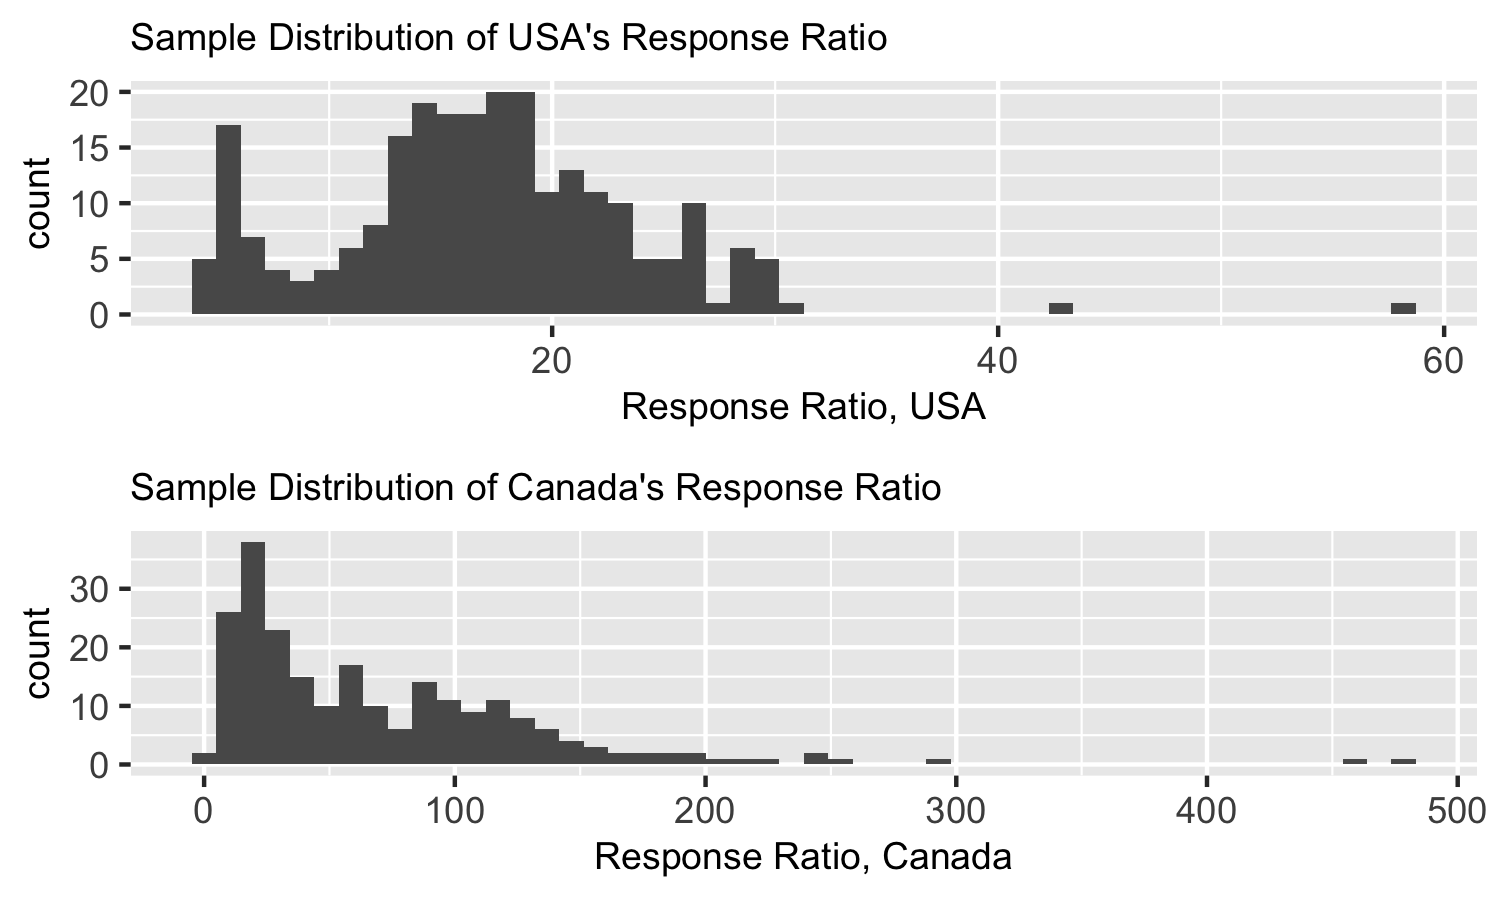
\includegraphics{../results/histogram_plot.png} Figure 1. Sample
Distribution of Daily Response Ratio for the USA and Canada between
March 1st 2020 and October 31st 2020.

We analyzed and confirmed that there is a difference in the variances of
distributions of the daily response ratio data for both Canada and the
USA during the time-line of interest through a Bartlett's test.

The team decided to use permutation based hypothesis testing to answer
our statistical question. We chose a 95\% confidence level for our
sample estimate i.e a significance threshold level of
\({\alpha = 0.05}\).

Our Null(\(H_0\)) and Alternate(\(H_a\)) Hypotheses are:

\[ \text {$H_0$: The median daily response ratio of Canada and the USA between March 1st 2020 and October 31st 2020 is equal} \]
\[ \text {$H_a$: The median daily response ratio of Canada and the USA between March 1st 2020 and October 31st 2020 is not equal} \]
We generated a bootstrap distribution of bootstrap sample median
response ratios for Canada and the USA during the time-line of interest.
We visualized our booststrap distributions as shown in the figure below.

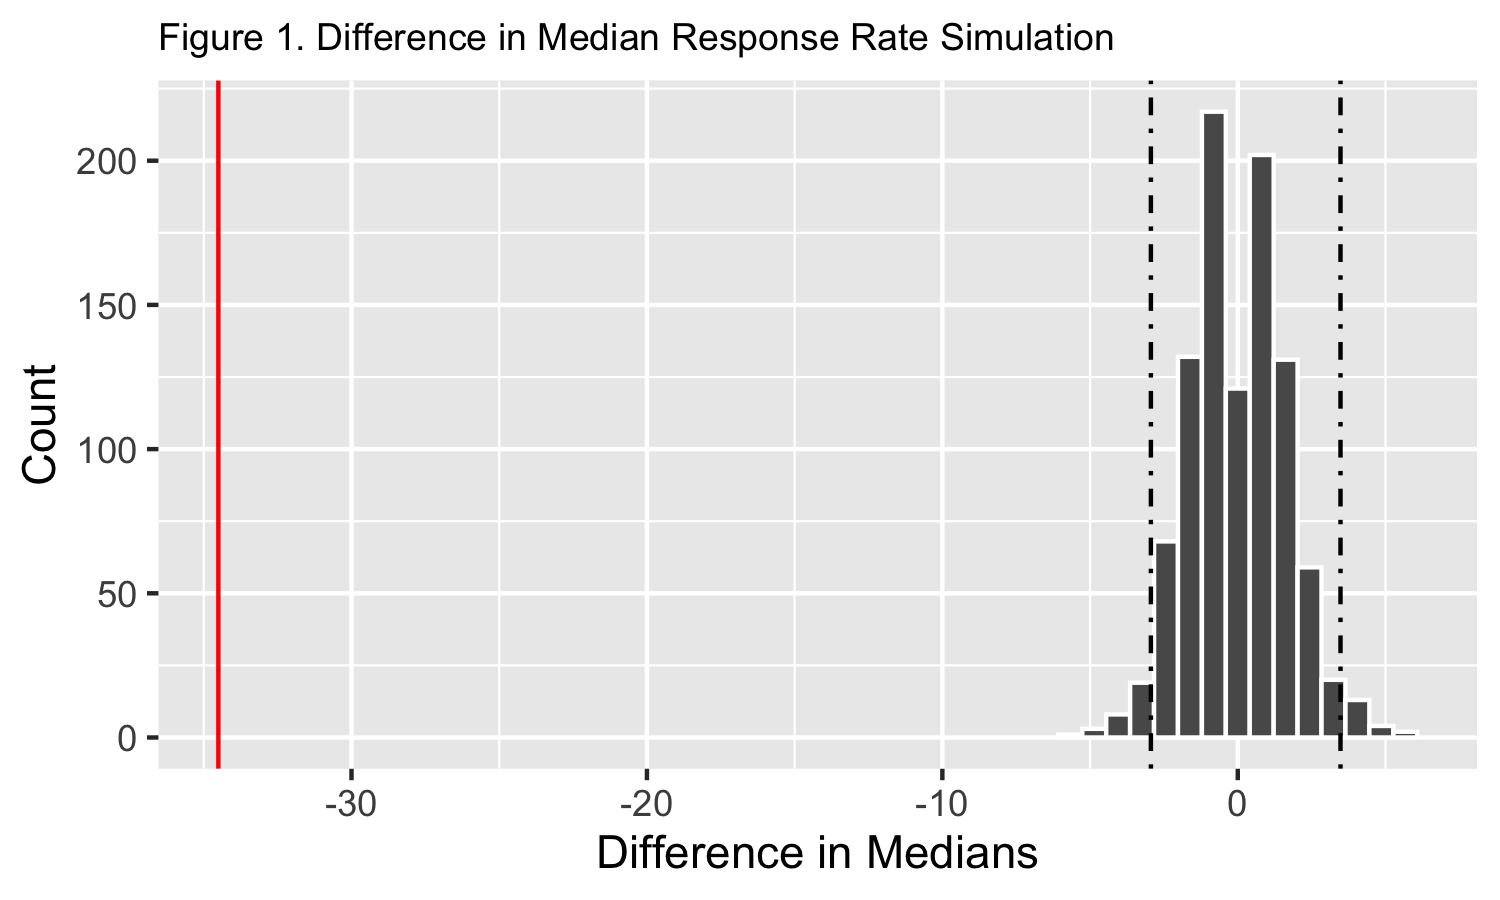
\includegraphics{../results/median_simulation.png} Figure 2. Simulation
based Bootstrap Distribution for the Null Hypothesis.

Thereafter, we calculated the p-value for our hypothesis test. The
results are discussed in the section below.

The R (R Core Team 2019) and Python (Van Rossum and Drake 2009)
programming languages were used to perform the analysis in this project.
Several R and Python packages were used, a complete list of package
dependencies can be found in the
\href{https://github.com/UBC-MDS/covid-19-cases-vs-tests-analysis/blob/main/README.md}{Readme.md}.
All the code used in the analysis can be found
\href{https://github.com/UBC-MDS/covid-19-cases-vs-tests-analysis/tree/main/src}{here}.

\hypertarget{results-and-discussion}{%
\section{Results and Discussion}\label{results-and-discussion}}

The p-value for our test was \textless0.0001 (Table 1). Based on this
p-value, since it is much lower than our significance threshold of 0.05
we reject our Null Hypothesis that the median daily response ratio of
Canada and the USA between March 1st 2020 and October 31st 2020 is
equal.

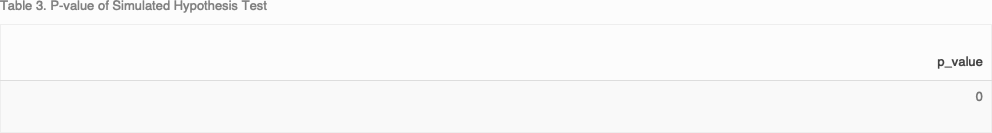
\includegraphics{../results/simulation_pval.png}

Table 1. p-value from the Permutation based Hypothesis Testing.

Based on our analysis we can-not categorically say that Canada's overall
response strategy towards COVID-19 was more efficient that that of the
USA; however, we can infer with reasonable confidence that the median
daily response ratio as defined within the confines of our earlier
stated assumptions was higher for Canada than the USA between March 1st
2020 and October 31st 2020.

We also acknowledge that there are some pitfalls such as selection-bias,
random-variability, and sampling-variability (Roger D. Peng 2016) which
our analysis doesn't address owing to the scope of the project as
explained earlier.

\hypertarget{future-work}{%
\section{Future Work}\label{future-work}}

Our analysis can be built upon further to devise a more sophisticated
framework to understand COVID-19 responses in Canada and the USA. Some
of the interesting points which would help expand the scope of this
project include:

\begin{enumerate}
\def\labelenumi{\arabic{enumi}.}
\tightlist
\item
  Include more robust data, for e.g.~finding data for some of the
  missing days in the current data set.
\item
  Expand the time-line of consideration for the analysis.
\item
  Address the auto-correlation caused by the temporal nature of the
  daily data points by using appropriate time-series analysis
  techniques.
\item
  Explore more features to include in quantifying the
  \texttt{Response\ Ratio}.
\item
  Build a model to take into account the other relevant features as
  discovered in the point above.
\end{enumerate}

\hypertarget{references}{%
\section*{References}\label{references}}
\addcontentsline{toc}{section}{References}

\hypertarget{refs}{}
\begin{cslreferences}
\leavevmode\hypertarget{ref-govCA}{}%
Canada, Government of. 2020. ``COVID-19 Situational Awareness
Dashboard.''
\url{https://health-infobase.canada.ca/covid-19/dashboard/}.

\leavevmode\hypertarget{ref-cdc}{}%
Disease Control, Centers for, and Prevention. 2020. ``COVID-19 Death
Data and Resources.''
\url{https://www.who.int/emergencies/diseases/novel-coronavirus-2019}.

\leavevmode\hypertarget{ref-first-case}{}%
Holshue, Michelle L., Chas DeBolt, Scott Lindquist, Kathy H. Lofy, John
Wiesman, Hollianne Bruce, Christopher Spitters, et al. 2020. ``First
Case of 2019 Novel Coronavirus in the United States.'' \emph{The New
England Journal of Medicine} 382 (10): 929--36.

\leavevmode\hypertarget{ref-covid-score}{}%
Lazarus, Jeffrey V., Scott Ratzan, Adam Palayew, Francesco C. Billari,
Agnes Binagwaho, Spencer Kimball, Heidi J. Larson, et al. 2020.
``COVID-Score: A Global Survey to Assess Public Perceptions of
Government Responses to Covid-19 (Covid-Score-10).'' \emph{PLoS One} 15
(10).
\url{https://ezproxy.library.ubc.ca/login?url=https://www-proquest-com.ezproxy.library.ubc.ca/docview/2448834819?accountid=14656}.

\leavevmode\hypertarget{ref-epidemiology}{}%
Li, Jie, Daniel Q. Huang, Biyao Zou, Hongli Yang, Wan Z. Hui, Fajuan
Rui, Natasha T. S. Yee, et al. 2020. ``Epidemiology of Covid‐19: A
Systematic Review and Meta‐analysis of Clinical Characteristics, Risk
Factors, and Outcomes.'' \emph{Journal of Medical Virology}.

\leavevmode\hypertarget{ref-owidcoronavirus}{}%
Max Roser, Esteban Ortiz-Ospina, Hannah Ritchie, and Joe Hasell. 2020.
``Coronavirus Pandemic (Covid-19).'' \emph{Our World in Data}.

\leavevmode\hypertarget{ref-who}{}%
Organization, World Health. 2020. ``Novel-Coronavirus-2019.''
\url{https://www.cdc.gov/nchs/nvss/vsrr/covid19/index.htm}.

\leavevmode\hypertarget{ref-R}{}%
R Core Team. 2019. \emph{R: A Language and Environment for Statistical
Computing}. Vienna, Austria: R Foundation for Statistical Computing.
\url{https://www.R-project.org/}.

\leavevmode\hypertarget{ref-aods}{}%
Roger D. Peng, Elizabeth Matsui. 2016. \emph{The Art of Data Science}.

\leavevmode\hypertarget{ref-Python}{}%
Van Rossum, Guido, and Fred L. Drake. 2009. \emph{Python 3 Reference
Manual}. Scotts Valley, CA: CreateSpace.
\end{cslreferences}

\end{document}
